\section{Lesende und rechnende Kassen: Von der Industrie- zur Konsumgesellschaft}

\subsection{Einführung: Technik im Übergang zur Konsumgesellschaft}

Die Vorlesung untersucht den historischen Übergang
von der Industriegesellschaft zur Konsumgesellschaft.

Während Technik im 19. und frühen 20. Jahrhundert
vor allem mit industrieller Produktion,
Fabriken und Arbeitsorganisation verbunden war,
verlagerte sie sich im Verlauf des 20. Jahrhunderts
zunehmend in den Alltag.

Technik organisierte nun nicht mehr nur Arbeit,
sondern auch Konsum,
Haushaltsführung,
Wohnformen und Geschlechterrollen.

Zentrale Leitfragen:

\begin{itemize}
\item Wie verändert Technik den Alltag ausserhalb der Fabrik?
\item Welche Rolle spielte der Haushalt im Übergang zur Konsumgesellschaft?
\item Wie entstanden neue Konsumnormen und Vorstellungen vom richtigen Leben?
\item Wie veränderten technische Geräte die Rolle der Hausfrau?
\item Was zeigt der Strichcode über Konsum und Rationalisierung in den 1970er Jahren?
\end{itemize}

Die Geschichte lesender und rechnender Kassen
ist daher nicht nur eine Geschichte technischer Innovation,
sondern auch eine Geschichte gesellschaftlicher Ordnung,
des Konsums und der Veränderung alltäglicher Praktiken.

\subsection{Die Frankfurter Küche als rationalisierter Privatraum}

Die Vorlesung knüpft anschliessend
an die Rationalisierung des Haushalts an.

Ein wichtiges Beispiel dafür ist erneut
die Frankfurter Küche.

Sie entstand im Zusammenhang
mit der Wohnreform der Neuen Sachlichkeit.

Diese Reformbewegung verfolgte das Ziel,
Wohnräume funktional,
zweckmässig und hygienisch zu gestalten.

Die Frankfurter Küche wurde ab den 1920er Jahren entwickelt
und verbreitete sich später auch ausserhalb Deutschlands,
besonders in den 1950er Jahren.

Sie übertrug Prinzipien des scientific management
auf den privaten Wohnraum.

Ziele waren:

\begin{itemize}
\item Entlastung der Hausarbeit
\item mehr Komfort
\item hygienische Verbesserung
\item effizientere Arbeitsabläufe
\item Modernisierung des Alltags
\end{itemize}

Besonders im Wohnungsbau für Arbeiterfamilien
galt funktionaler Wohnungsbau
als erstrebenswerte Verbesserung
der Wohn- und Lebensverhältnisse.

\begin{center}
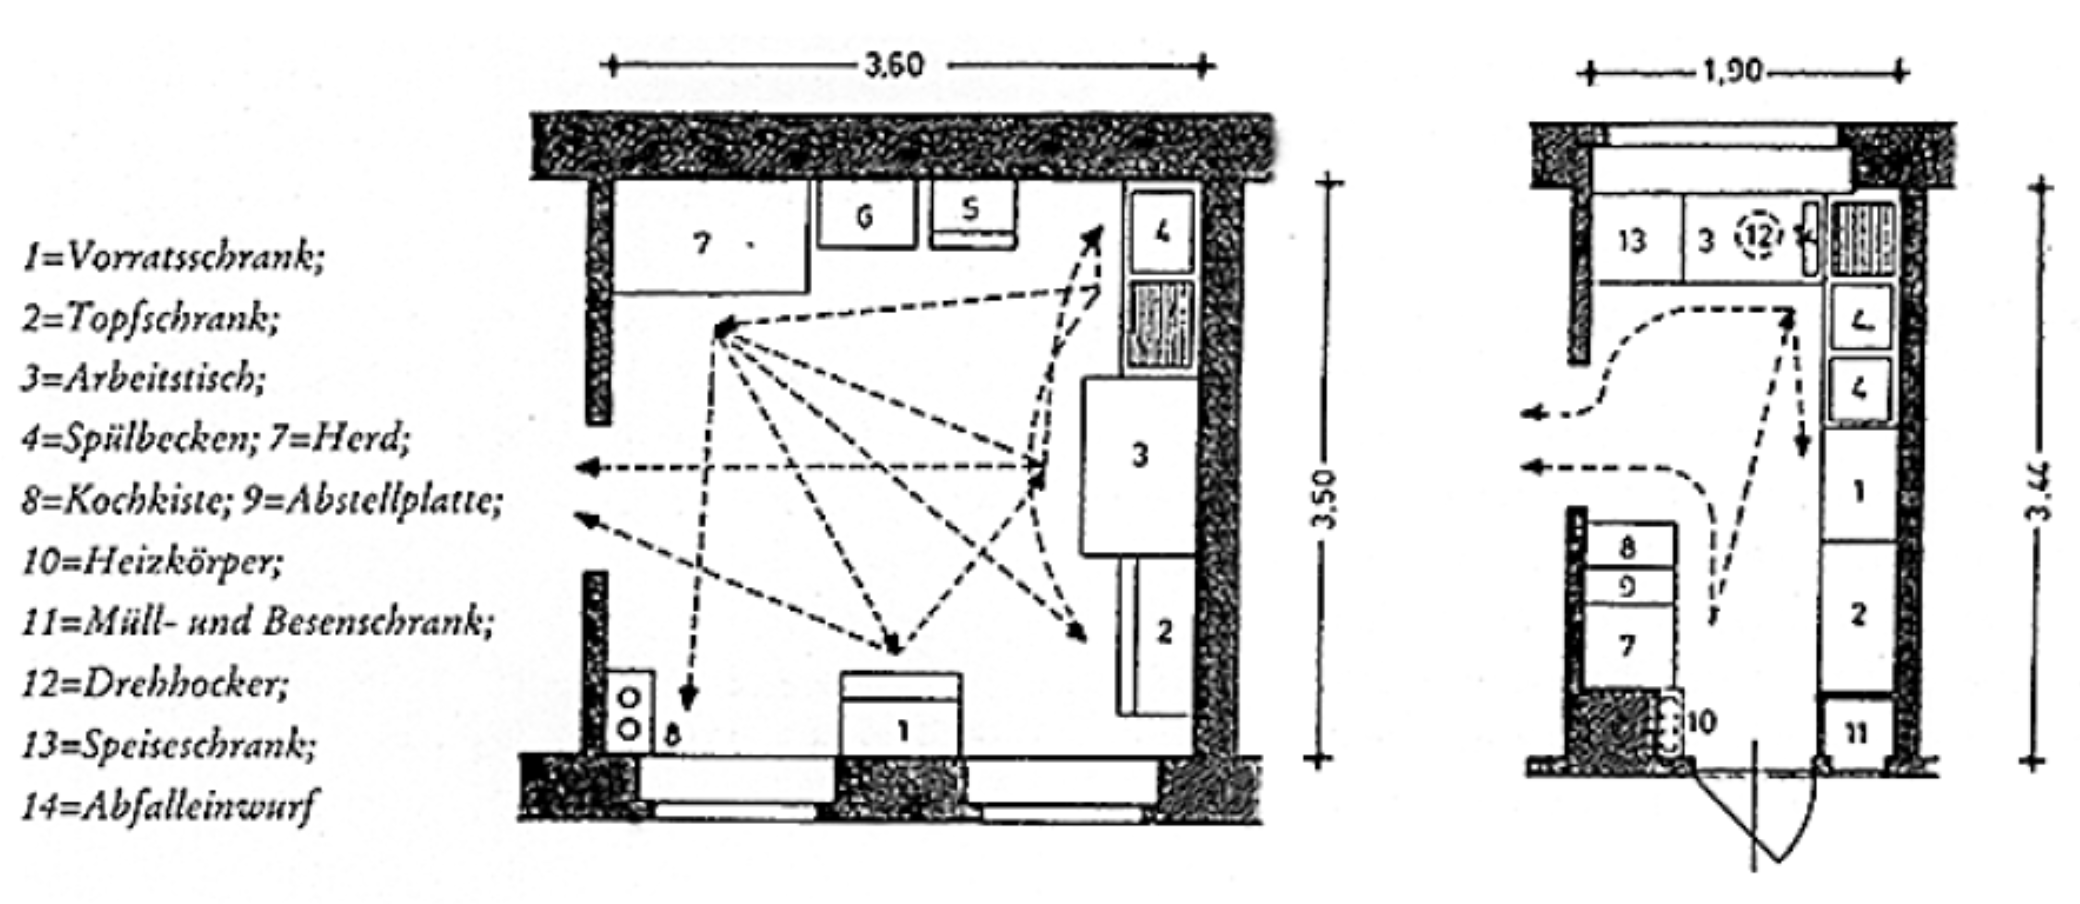
\includegraphics[width=0.85\linewidth]{images/frankfurter_kueche.png}
\end{center}

\subsection{Die Küche, das Heim und die Hausfrau}

Das neue Wohnkonzept ordnete jedem Raum
eine bestimmte Funktion zu.

Damit wurde nicht nur festgelegt,
wie Räume genutzt werden sollten,
sondern auch,
wer sich in ihnen aufhalten sollte.

Die Frankfurter Küche war als Arbeitsraum
für eine einzelne Person konzipiert.

Diese Person war in der gesellschaftlichen Vorstellung
die Hausfrau.

Die Architektur zwang die Bewohnerinnen und Bewohner
zwar nicht unmittelbar dazu,
entsprechend dieser Ordnung zu leben.

Sie legte jedoch bestimmte Verhaltensweisen nahe.

Die Küche wurde dadurch zu einem Raum,
in dem sich gesellschaftliche Vorstellungen
von Geschlecht,
Arbeit und Ordnung materialisierten.

Wichtig ist jedoch:
Die Figur der Frau als Managerin des Haushalts
entstand nicht erst durch diese baulichen Massnahmen.

Sie existierte bereits zuvor
und wurde durch die neue Wohnarchitektur
weiter stabilisiert.

\subsection{Der „Oikos“ als vormoderner Haushalt}

Um die moderne Hausfrau historisch einordnen zu können,
blickt die Vorlesung auf den vormodernen Haushalt zurück.

Vor der Industrialisierung,
also bis ins 18. Jahrhundert,
war der Haushalt nicht nur Wohnort,
sondern zugleich Arbeitsstätte.

Er bildete eine kleine,
relativ ganzheitliche Wirtschaftseinheit.

Der Haushalt war weitgehend auf Selbstversorgung ausgerichtet.

Viele Dinge,
die für das tägliche Leben gebraucht wurden,
wurden selbst hergestellt oder produziert.

Dazu gehörten unter anderem:

\begin{itemize}
\item Feldarbeit
\item Ernte
\item Viehhaltung
\item Nähen von Kleidern
\item Waschen und Putzen
\item Kochen
\item Haltbarmachen von Lebensmitteln
\end{itemize}

Auch in der Vormoderne waren Arbeiten
geschlechtlich zugeordnet.

Dennoch beteiligten sich grundsätzlich
alle im Haushalt lebenden Personen
in irgendeiner Form an der Hausarbeit.

Der Hausherr repräsentierte den Haushalt nach aussen,
während die Hausmutter die Arbeit organisierte.

\begin{center}
\includegraphics[width=0.5\linewidth]{images/oikos.png}
\end{center}

\subsection{Die Hausfrau als Erfindung des 19. Jahrhunderts}

Mit der Industrialisierung veränderte sich
die Struktur des Haushalts grundlegend.

Produktion und Reproduktion wurden zunehmend getrennt.

Die Fabrik wurde zum Ort der Erwerbsarbeit,
das Haus zum Ort der Reproduktion,
Kindererziehung und Haushaltsführung.

Dadurch entstanden ein öffentlicher
und ein privater Raum,
die klar voneinander unterschieden wurden.

Als gesellschaftliche Norm setzte sich zunehmend
folgendes Familienmodell durch:

\begin{itemize}
\item Der Mann arbeitet ausser Haus als Lohnarbeiter oder Erwerbstätiger.
\item Er gilt als Ernährer der Familie.
\item Die Frau bleibt im Haus.
\item Sie zieht die Kinder auf und führt den Haushalt.
\end{itemize}

Die Arbeit der Frau und Mutter
wurde dabei nicht entlohnt.

Gleichzeitig wurde sie moralisch stark aufgeladen.

Die gute Hausfrau wurde zum Ideal
einer geordneten,
modernen und bürgerlichen Lebensweise.

\subsection{Technisierung des Haushalts ab den 1920er Jahren}

Ab den 1920er Jahren kamen vermehrt technische Geräte
für den Haushalt auf den Markt.

Dazu gehörten:

\begin{itemize}
\item Staubsauger
\item Backöfen
\item Waschmaschinen
\item elektrische Lampen
\item weitere elektrische Haushaltsgeräte
\end{itemize}

Als Konsumgüter für breite Bevölkerungsschichten
wurden diese Geräte jedoch erst nach dem Zweiten Weltkrieg
wirklich erschwinglich.

Mit technischen Geräten sollte der Haushalt
effizienter geführt werden.

Ähnlich wie in der Fabrik
kam es auch im Haushalt
zu einer Reorganisation von Arbeit.

Die Technisierung brachte neue Normen,
Zielsetzungen und Erwartungen hervor.

Der Haushalt sollte sauberer,
moderner,
rationeller und besser organisiert sein.

\begin{center}
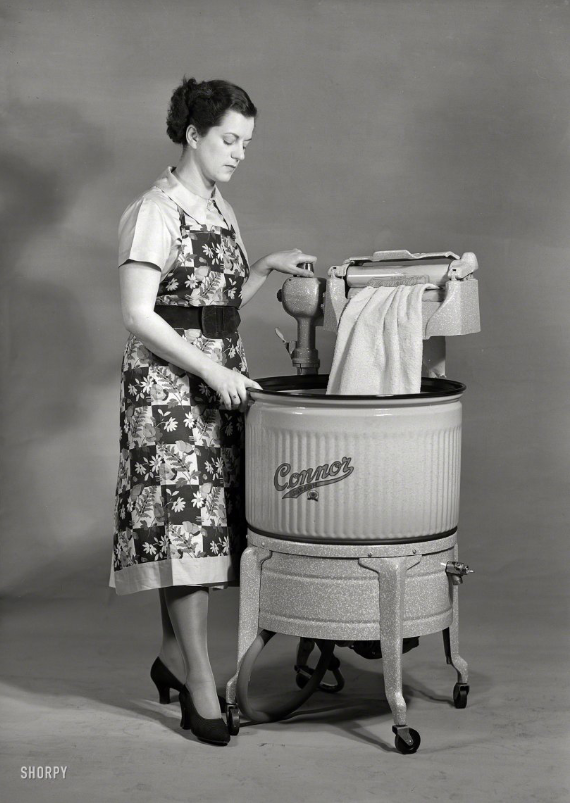
\includegraphics[width=0.5\linewidth]{images/Technik_im_Haushalt.png}
\end{center}

\subsection{Entlastung, Isolation und Geschlechterrollen}

Technische Geräte versprachen zunächst
eine deutliche Entlastung.

Sie konnten körperlich anstrengende Arbeiten
vereinfachen oder beschleunigen.

Besonders die Hausfrau sollte dadurch
von schwerer körperlicher Arbeit entlastet werden.

Gleichzeitig führte die Technisierung des Haushalts
aber auch zu neuen Formen der Isolation.

Hausarbeit wurde weniger in Kooperation
und Gemeinschaft verrichtet.

Stattdessen arbeitete die Hausfrau zunehmend allein
mit technischen Geräten im privaten Raum.

Technik stabilisierte damit bestehende Geschlechterrollen.

Sie machte den Haushalt effizienter,
stellte aber die geschlechtliche Zuständigkeit
für diese Arbeit nicht grundsätzlich in Frage.

Die Vorlesung betont jedoch,
dass die Stabilisierung von Geschlechterrollen
durch Technik kontextabhängig ist.

Technik besitzt kein festes Geschlecht.

Ihre gesellschaftliche Bedeutung entsteht erst
durch konkrete Arbeitsverhältnisse,
Eigentumsformen,
Körperbilder und kulturelle Zuschreibungen.

%\begin{center}
%\includegraphics[width=0.65\linewidth]{images/waschmaschine_1950.png}
%\end{center}

\subsection{Technik und Geschlecht}

Die Vorlesung zeigt anhand verschiedener Beispiele,
dass Geschlecht \textbf{nicht} einfach in Technik eingeschrieben ist.

Technische Geräte sind \textbf{nicht} von sich aus männlich oder weiblich.

Erst ihre Nutzung,
ihre soziale Einbettung
und ihre ökonomische Bedeutung
machen sie zu geschlechtlich codierten Objekten.

Beim Maschinensticken führte der Einsatz von Maschinen dazu,
dass Männer in einem Bereich tätig wurden,
der zuvor stark mit weiblicher Handarbeit verbunden war.

Dies hing unter anderem damit zusammen,
dass Maschinensticken kapitalintensiv war
und Besitz,
Wartung und körperliche Belastung erforderte.

Bei der Schreibarbeit verlief die Entwicklung anders.

Durch die Schreibmaschine wurde Büro- und Sekretariatsarbeit
zunehmend feminisiert.

Diese Arbeit wurde zugleich abgewertet
und schlechter entlohnt.

Daran zeigt sich:

Nicht die Technik selbst bestimmt Geschlechterrollen,
sondern ihre gesellschaftliche Organisation.

%\begin{center}
%\includegraphics[width=0.8\linewidth]{images/technik_und_geschlecht.png}
%\end{center}

\subsection{Technisierung des Haushalts ab den 1950er Jahren}

Ab den 1950er Jahren wurden technische Geräte
zunehmend zu Konsumgütern.

Der Haushalt wurde dadurch zu einem wichtigen Markt.

Die durch Technik stabilisierte Figur der Hausfrau
wurde nun zugleich zur Konsumentin.

Werbung und Produktdesign richteten sich
an ihre vermeintlichen Bedürfnisse.

Gleichzeitig schufen sie diese Bedürfnisse
aber auch erst mit.

Waschmittel,
Küchengeräte,
Staubsauger,
Kühlschränke und andere Produkte
wurden nicht nur als praktische Hilfen verkauft,
sondern als Zeichen eines modernen,
richtigen und gepflegten Haushalts.

Dadurch entstanden neue Normen darüber,
wie ein Haushalt geführt werden sollte.

Besonders wichtig wurden Erwartungen an:

\begin{itemize}
\item Hygiene
\item Sauberkeit
\item Ausstattung
\item Ordnung
\item Dekoration
\item Modernität
\end{itemize}

Die Hausfrau wurde damit zur zentralen Figur
der Konsumgesellschaft.

Sie war verantwortlich für den Kauf,
die Nutzung und die Bewertung technischer Konsumgüter
im privaten Alltag.

%\begin{center}
%\includegraphics[width=0.55\linewidth]{images/persil_werbung_1950er.png}
%\end{center}

\subsection{Der Strichcode und die Rationalisierung des Konsums}

Ein weiteres Thema der Vorlesung ist der Strichcode,
der in den 1970er Jahren
als neue Kassentechnologie diskutiert wurde.

Die Quelle zum Strichcode von 1973 zeigt,
wie technische Rationalisierung
auch den Bereich des Einkaufens erfasste.

Die Kasse wurde nicht mehr nur als Ort des Bezahlens verstanden,
sondern als Schnittstelle zwischen Ware,
Information,
Preis,
Verkauf und Konsumverhalten.

Der Strichcode versprach:

\begin{itemize}
\item schnelleres Kassieren
\item genauere Preisberechnung
\item bessere Warenkontrolle
\item effizientere Lagerhaltung
\item Rationalisierung des Detailhandels
\end{itemize}

Damit wurde eine Logik,
die zuvor vor allem aus Fabrik und Verwaltung bekannt war,
auf den Konsum übertragen.

Nicht nur die Produktion,
sondern auch der Einkauf wurde messbar,
standardisiert und berechenbar.

Die lesende und rechnende Kasse steht daher
für eine neue Phase der Konsumgesellschaft.

Konsum wurde technisch organisiert,
statistisch erfassbar
und ökonomisch besser steuerbar.
\begin{center}
\includegraphics[width=0.8\linewidth]{images/barcode.png}
\end{center}

\subsection{Von der Industrie- zur Konsumgesellschaft}

Die zentrale These der Vorlesung lautet,
dass sich Technik im 20. Jahrhundert
zunehmend vom industriellen Produktionsbereich
in den Alltag verlagerte.

In der Industrie organisierte Technik Arbeit.

Im Haushalt organisierte sie Lebensweisen,
Konsumpraktiken und Geschlechterrollen.

Die Hausfrau war ein Produkt der Moderne.

Sie stand im Zentrum eines technisierten Alltags,
der weniger auf Produktion
als auf Konsum und Reproduktion ausgerichtet war.

Technische Geräte,
Werbung,
Produktdesign,
Wohnarchitektur und Kassensysteme
wirkten gemeinsam an der Entstehung
moderner Konsumgesellschaften mit.

In der Konsumgesellschaft wurden Technik
und Technikfolgen zudem zunehmend
zu Themen des öffentlichen Lebens und der Politik.

Dazu gehörten Fragen nach:

\begin{itemize}
\item Umwelt
\item Infrastruktur
\item Deindustrialisierung
\item Konsumkritik
\item sozialer Ordnung
\end{itemize}

\subsection{Zentrale Erkenntnisse}

Die Vorlesung zeigt,
dass Technik nicht nur Maschinenarbeit
in Fabriken veränderte.

Sie prägte auch den privaten Alltag,
die Organisation des Haushalts
und die Entstehung moderner Konsumformen.

Zentrale Erkenntnisse sind:

\begin{itemize}
\item Die moderne Hausfrau entstand im Zusammenhang mit der Trennung von Produktion und Reproduktion.
\item Haushaltsgeräte versprachen Entlastung, stabilisierten aber häufig bestehende Geschlechterrollen.
\item Technik ist nicht von sich aus geschlechtlich, sondern wird in bestimmten sozialen Kontexten geschlechtlich codiert.
\item Ab den 1950er Jahren wurde der Haushalt zu einem zentralen Ort des Konsums.
\item Werbung und Produktdesign schufen neue Bedürfnisse und Normen des richtigen Haushalts.
\item Der Strichcode zeigt, wie Rationalisierung auch den Einkauf und den Konsum erfasste.
\end{itemize}

Die zentrale These lautet:

Der Übergang von der Industrie- zur Konsumgesellschaft
bedeutete nicht das Ende technischer Rationalisierung.

Vielmehr verlagerte sie sich in neue Bereiche.

Technik strukturierte nun nicht mehr nur Produktion und Arbeit,
sondern auch Konsum,
Haushalt,
Geschlechterrollen und alltägliche Lebensführung.
